\documentclass[11pt,a4paper]{article}

\usepackage[utf8]{inputenc}
\usepackage[T1]{fontenc}
\usepackage[english]{babel}
\usepackage{geometry}
\geometry{margin=2.5cm}
\usepackage{amsmath,amssymb}
\usepackage{booktabs}
\usepackage{array}
\usepackage{tikz}
\usetikzlibrary{calc,arrows.meta}
\usepackage[hidelinks]{hyperref}
\numberwithin{equation}{section}

\newcommand{\bs}[1]{\boldsymbol{#1}}
\newcommand{\T}{^{\mathsf T}}
\newcommand{\code}[1]{\texttt{#1}}

\hypersetup{
  pdftitle={Rigid-body 2-DOF gimbal model -- Mathematical summary},
  pdfauthor={Alessandro Curci}
}

\title{Rigid-Body Dynamic Model of an Alt-Azimuth\\ Telescope Mount\\[4pt]
\large Mathematical Summary, Verified Against the Implementation}
\author{Alessandro Curci}
\date{September 28, 2026}

\begin{document}
\maketitle

\begin{abstract}
\noindent This note is a self-contained mathematical summary of the rigid two-degree-of-freedom model (azimuth~$\psi$, elevation~$\theta$) of the alt-azimuth mount specified in \texttt{SPEC\_\allowbreak modello\_\allowbreak gimbal\_\allowbreak 2dof.md} and implemented in \texttt{src/gimbal/}. Unlike a paraphrase of the specification, every formula and every number below has been checked against the actual symbolic output of the code (\texttt{results/latex/eom.tex}, \texttt{results/latex/tf.tex}) and against the numeric results of a full run (\texttt{results/report.md}, \texttt{results/tables/inertia\_summary.csv}) with the confirmed configuration (\texttt{config.yaml}, \texttt{z\_O\_cm = 54.9}). Two places where the specification stated a narrower result than what the code actually proves have been corrected directly in the specification (Section~2 and Section~7 of that file); they are also explained here. The document gives particular attention to how the eccentricity between the rotation axes and the telescope's center of mass enters the model -- in the inertia tensor, in the potential energy, and in the linearized stiffness -- and closes with a section on how the nonlinear and linearized problems are actually solved numerically.
\end{abstract}

\tableofcontents
\newpage

\section{Purpose and provenance of this document}
\label{sec:intro}

This document follows one rule throughout: \textbf{the implementation is the source of truth}. Where the specification and the code agreed, the corresponding formula is simply restated. Where a value in the specification was an idealized test fixture rather than the real configured mount (Section~\ref{subsec:d-vector}), or where the code proves a stronger, more general result than the specification claims (Section~\ref{subsec:lin-matrici}), this is flagged explicitly and the specification file has been corrected. No formula below was hand-derived and then assumed correct; every one was cross-checked either against \texttt{results/latex/eom.tex} / \texttt{tf.tex} (the literal \texttt{SymPy} output) or against a passing test in \texttt{tests/}.

As stated in the code's own realism note (\texttt{README.md}, \texttt{results/report.md}): this is a two-rigid-body model. It contains no structural modes. The only nontrivial dynamics it can produce are a low-frequency rigid-body behavior driven by gravity (imbalance), gyroscopic coupling, and centrifugal stiffening -- typically below 1\,Hz. Section~\ref{sec:realismo} gives the real, computed numbers behind this statement, not just the general claim.

\section{Reference Frames, Geometry, and Kinematics}
\label{sec:cinematica}

\subsection{Frames, and why there are two of them}
\label{subsec:frames}

Four frames are used:
\begin{itemize}
\item $W$: the CAD assembly frame. This is not a frame the model chooses -- it is fixed by Onshape's \emph{Mass properties} tool, whose origin is the center of the base of the azimuth shaft, with $Z_W$ vertical. Every raw number in the specification (centers of mass, inertia tensors) is reported in $W$ because that is what the CAD tool exports.
\item $N$: the frame the Lagrangian mechanics is written in, with origin at $O$ (the intersection of the azimuth and elevation axes) and $Z_N = Z_W$.
\item $A$: the fork, rotated by $\psi$ about $Z$ relative to $N$.
\item $B$: the telescope, with pointing axis $x_B$, elevation axis $y_B$, and $z_B = x_B \times y_B$.
\end{itemize}

\paragraph{Why two frames, and why $N$ needs no rotation matrix of its own.}
$W$ and $N$ exist for different reasons: $W$ is where the data \emph{comes from}, $N$ is where the dynamics is \emph{naturally written} -- centered on the physical pivot $O$ that both rotations pass through, not on an arbitrary CAD origin. Because the azimuth axis is vertical and passes through the origin of $W$ by construction, and $O$ lies on that same vertical line at height $z_O$, \textbf{$N$ and $W$ share exactly the same orientation}: $N$ is $W$ translated vertically by $z_O$, nothing more. This is not an approximation; it is confirmed directly by \texttt{params.py}, which never builds a rotation matrix between $W$ and $N$ at all -- it only ever builds a translation $\bs r_O|_W$ (Eq.~\eqref{eq:rO}) and the rotations $\bs R_{WA0}, \bs R_{WB0}$ that go \emph{directly} from $W$ into the fork and telescope body frames. Every quantity "in $N$" used later (the transported inertia tensor, the eccentricity vector) is, in the actual implementation, simply "in $W$-aligned axes, taken about the point $O$" -- valid precisely because no rotation separates $W$ from $N$.

The orientation of $B$ relative to $N$ is
\begin{equation}
\bs R_{NB} = \bs R_z(\psi)\,\bs R_y(\theta),
\qquad
\bs R_y(\theta) = \begin{bmatrix}\cos\theta & 0 & \sin\theta\\ 0&1&0\\ -\sin\theta & 0 & \cos\theta\end{bmatrix},
\qquad
\bs R_z(\psi) = \begin{bmatrix}\cos\psi & -\sin\psi & 0\\ \sin\psi&\cos\psi&0\\ 0&0&1\end{bmatrix},
\label{eq:RNB}
\end{equation}
exactly as implemented in \texttt{kinematics.R\_NB} and \texttt{params.R\_NB}.

\subsection{Geometry at a glance}
\label{subsec:diagram}

\begin{figure}[htbp]
\centering
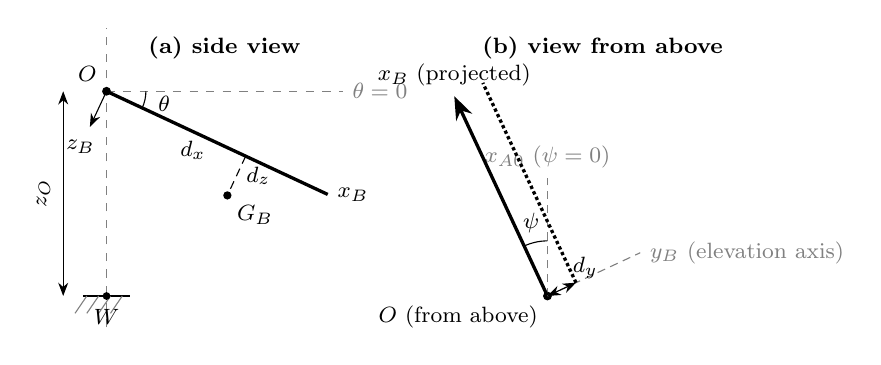
\begin{tikzpicture}[>=Stealth, every node/.style={font=\footnotesize}]
  % ===================== Panel A: side (elevation) view =====================
  \begin{scope}
    \draw[dashed, gray] (0,-0.4) -- (0,3.4);
    \draw[thick] (-0.3,0) -- (0.3,0);
    \foreach \x in {-0.25,-0.1,0.05,0.2} {\draw[gray] (\x,0) -- (\x-0.15,-0.22);}
    \fill (0,0) circle (1.4pt);
    \node[below] at (0,-0.05) {$W$};
    \coordinate (O) at (0,2.6);
    \fill (O) circle (1.6pt);
    \node[above left] at (O) {$O$};
    \draw[<->] (-0.55,0) -- (-0.55,2.6);
    \node[rotate=90] at (-0.8,1.3) {$z_O$};
    \draw[dashed, gray] (O) -- ++(3.0,0);
    \node[right, gray] at ($(O)+(3.0,0)$) {$\theta=0$};
    \pgfmathsetmacro{\thetadraw}{-25}
    \coordinate (xBtip) at ($(O)+(\thetadraw:3.1)$);
    \draw[very thick] (O) -- (xBtip);
    \node[right] at (xBtip) {$x_B$};
    \draw ($(O)+(0.5,0)$) arc (0:\thetadraw:0.5);
    \pgfmathsetmacro{\thetalabang}{\thetadraw/2}
    \node at ($(O)+(\thetalabang:0.75)$) {$\theta$};
    \coordinate (P) at ($(O)+(\thetadraw:1.95)$);
    \draw[densely dashed] (O) -- (P);
    \pgfmathsetmacro{\perpang}{\thetadraw-90}
    \coordinate (GB) at ($(P)+(\perpang:0.55)$);
    \draw[densely dashed] (P) -- (GB);
    \fill (GB) circle (1.5pt);
    \node[below right] at (GB) {$G_B$};
    \node[below] at ($(O)!0.62!(P)$) {$d_x$};
    \node[right] at ($(P)!0.5!(GB)$) {$d_z$};
    \draw[->] (O) -- ($(O)+(\perpang:0.5)$);
    \node at ($(O)+(\perpang:0.78)$) {$z_B$};
    \node at (1.5,3.15) {\textbf{(a) side view}};
  \end{scope}

  % ===================== Panel B: top view =====================
  \begin{scope}[xshift=5.6cm]
    \coordinate (Otop) at (0,0);
    \fill (Otop) circle (1.6pt);
    \node[below left] at (Otop) {$O$ (from above)};
    \draw[densely dashed, gray] (Otop) -- (0,1.5);
    \node[above, gray] at (0,1.5) {$x_{A0}$ ($\psi=0$)};
    \pgfmathsetmacro{\psidraw}{25}
    \pgfmathsetmacro{\xBangle}{90+\psidraw}
    \coordinate (xBtopTip) at ($(Otop)+(\xBangle:2.8)$);
    \draw[very thick,->] (Otop) -- (xBtopTip);
    \node[above] at (xBtopTip) {$x_B$ (projected)};
    \draw (0,0.7) arc (90:\xBangle:0.7);
    \pgfmathsetmacro{\psilabang}{90+\psidraw/2}
    \node at ($(\psilabang:0.95)$) {$\psi$};
    \pgfmathsetmacro{\yBangle}{\xBangle-90}
    \draw[densely dashed, gray] (Otop) -- ($(Otop)+(\yBangle:1.3)$);
    \node[right, gray] at ($(Otop)+(\yBangle:1.3)$) {$y_B$ (elevation axis)};
    \coordinate (shift) at ($(\yBangle:0.4)$);
    \coordinate (Tstart) at ($(Otop)+(shift)$);
    \coordinate (Tend) at ($(xBtopTip)+(shift)$);
    \draw[very thick, densely dotted] (Tstart) -- (Tend);
    \draw[<->] (Otop) -- (Tstart);
    \node[above right] at ($(Otop)!0.55!(Tstart)$) {$d_y$};
    \node at (0.7,3.15) {\textbf{(b) view from above}};
  \end{scope}
\end{tikzpicture}
\caption{Schematic geometry (not to scale; offsets exaggerated for legibility). \textbf{(a)} Side view: the azimuth axis is vertical, passing through the $W$ origin (base of the azimuth shaft) and through $O$, at height $z_O$ above it. At elevation $\theta$, the eccentricity vector $\bs d$ decomposes, in the vertical plane, into $d_x$ (along the pointing axis $x_B$) and $d_z$ (perpendicular to it); only these two components load the potential energy, Eq.~\eqref{eq:V}. \textbf{(b)} View looking down the azimuth axis: $x_{A0}$ is the fork's reference direction at $\psi=0$; the solid arrow is the actual pointing direction at azimuth $\psi$, with the (co-rotating) elevation axis $y_B$ perpendicular to it. The dotted line is the telescope's actual centerline, offset from the line through $O$ by $d_y$ -- a purely horizontal offset that never changes the center of mass's height, which is why $d_y$ is absent from $V$ (Section~\ref{subsec:V}) even though it is not zero (Section~\ref{subsec:d-vector}).}
\label{fig:geometria}
\end{figure}

Figure~\ref{fig:geometria} fixes the picture behind every formula that follows: point $O$ is the mechanical pivot; the eccentricity vector $\bs d$ is the offset of the telescope's center of mass from it, and only its components in the vertical plane of the current elevation angle ($d_x$, $d_z$) can ever produce a gravity torque, because rotating about the vertical azimuth axis or shifting along the (always-horizontal) elevation axis $y_B$ cannot change the height of the center of mass.

\subsection{Generalized coordinates, angles, and torques}
\label{subsec:angoli}

The generalized coordinates are $\bs q = [\psi,\ \theta]\T$. By the binding convention of the specification, $\theta>0$ lowers the pointing direction (right-hand rule about $y_B$): $\theta=0$ is the horizon, $\theta=-90^\circ$ the zenith. The physical elevation $\varepsilon=-\theta$ is used only for plot labels. $\psi$ is positive counterclockwise viewed from above. The generalized torques $\tau_\psi,\tau_\theta$ are defined by the virtual work
\begin{equation}
\delta W = \tau_\psi\,\delta\psi + \tau_\theta\,\delta\theta .
\end{equation}
The confirmed operating range of the real mount is $\theta \in [-45^\circ, 45^\circ]$ (user-confirmed 2026-09-27) -- not the full kinematic domain $[-90^\circ,0^\circ]$ -- and this restriction matters: several quantities below (notably $J_\psi(\theta)$, Section~\ref{subsec:eccentricity-in-azimuth}) behave differently over the confirmed range than over the full domain.

\subsection{Angular velocity}

The angular velocity of $B$ expressed in $B$ follows from Poisson's formula,
\begin{equation}
[\bs\omega_B|_B]_\times = \bs R_{NB}\T\,\dot{\bs R}_{NB},
\end{equation}
and \texttt{kinematics.verifica\_poisson} confirms by symbolic computation that it equals the closed form obtained by composing the two elementary rotations:
\begin{equation}
\bs\omega_B\big|_B = \bs R_y(\theta)\T\begin{bmatrix}0\\0\\\dot\psi\end{bmatrix} + \begin{bmatrix}0\\\dot\theta\\0\end{bmatrix}
= \begin{bmatrix}-\dot\psi\sin\theta\\ \dot\theta\\ \dot\psi\cos\theta\end{bmatrix}.
\label{eq:omegaB}
\end{equation}

\section{Inertial Properties and the Eccentricity Vector}
\label{sec:inerzia}

This section introduces point $O$ and the vector that measures how far the telescope's center of mass sits from it. That vector -- the \emph{eccentricity} -- is the single geometric fact that everything else (gravity torque, linearized stiffness, part of the inertia coupling) is built from.

\subsection{Point $O$ and the eccentricity vector}

With $x_{az}=y_{az}=0$ exactly by construction (the azimuth axis passes through the origin of $W$) and $z_O$ measured on the CAD,
\begin{equation}
\bs r_O\big|_W = (x_{az},\,y_{az},\,z_O), \qquad z_O = 54.9\ \text{cm (confirmed, config.yaml)}.
\label{eq:rO}
\end{equation}
In the CAD pose ($\psi=0$, $\theta=\theta_{CAD}=0$), the eccentricity vector is
\begin{equation}
\bs r = \bs r_{G_B} - \bs r_O \Big|_W ,
\label{eq:r-ecc}
\end{equation}
the segment joining the rotation axis to the telescope's center of mass -- the primitive geometric input that both the inertia correction (Section~\ref{subsec:huygens}) and the gravity term (Section~\ref{subsec:V}) are built from.

\subsection{Inertia transport: the tensorial Huygens--Steiner theorem}
\label{subsec:huygens}

The inertia tensor of $B$, known about its own center of mass as $\bs I_{B,G}|_W$, is transported to $O$ by
\begin{equation}
\bs I_{B,O}\big|_W = \bs I_{B,G}\big|_W + m_B\left(\lVert\bs r\rVert^2\,\mathbb 1 - \bs r\,\bs r\T\right),
\label{eq:huygens}
\end{equation}
implemented verbatim in \texttt{inertia.trasporta}, then rotated into the telescope's body frame,
\begin{equation}
\bs I_{B,O}\big|_B = \bs R_{WB0}\T\,\bs I_{B,O}\big|_W\,\bs R_{WB0}.
\label{eq:IBO-B}
\end{equation}
Its six components $I_{xx},I_{yy},I_{zz},I_{xy},I_{xz},I_{yz}$ (tensorial convention, $I_{ij}=-\int x_ix_j\,dm$ for $i\ne j$) are what enters the kinetic energy and the mass matrix from here on.

\subsection{The eccentricity vector in the body frame: real numbers}
\label{subsec:d-vector}

Projecting \eqref{eq:r-ecc} into frame $B$ gives the eccentricity vector as actually used by the dynamics,
\begin{equation}
\bs d = (d_x,\,d_y,\,d_z) = \bs R_{WB0}\T\,\bs r ,
\label{eq:d-def}
\end{equation}
(\texttt{inertia.\allowbreak costruisci\_\allowbreak modello\_\allowbreak inerziale}, step 6). With the confirmed configuration this evaluates, exactly, to
\begin{equation}
\bs d = (+7.965,\ +1.369,\ -0.440)\ \text{cm} = (+0.07965,\ +0.01369,\ -0.00440)\ \text{m}.
\label{eq:d-numeric}
\end{equation}
\emph{All three components are nonzero.} Physically:
\begin{itemize}
\item $d_x$ is the offset along the pointing axis $x_B$ -- the dominant term, roughly 8\,cm, coming directly from $y_{G_B}=-7.965$\,cm in the CAD pose (pointing along $-Y$);
\item $d_z$ is the small (4.4\,mm) offset perpendicular to the pointing axis, in the vertical plane;
\item $d_y = 1.369$\,cm is the offset along the elevation axis $y_B$ -- \emph{it is not zero}, but it has no effect on the potential energy (Section~\ref{subsec:V}), because $y_B$ stays horizontal for every $\psi,\theta$ (Figure~\ref{fig:geometria}b). It is not, however, dynamically inert: Section~\ref{subsec:eccentricity-in-M} shows exactly where it does act.
\end{itemize}
This is the vector the specification calls the \emph{eccentricity between the rotation axis and the center of mass}. Note that $\bs d$, not the raw CAD vector $\bs r$, is what appears in every dynamical equation from here on -- it is $\bs r$ expressed in the frame that actually rotates with the telescope.

\paragraph{A caution about "reference" numbers.} The specification's Section~5 table of expected values was computed at a \emph{different}, idealized configuration (\texttt{z\_O\_cm = null}, forcing $d_z=0$ exactly) used purely to unit-test the code, independently of whatever is later confirmed in \texttt{config.yaml} (\texttt{results/report.md}, Section~5: "\emph{I valori attesi... si riferiscono alla configurazione di riferimento... così da verificare il codice indipendentemente dalle scelte fatte in config.yaml}"). The real, confirmed mount has $z_O=54.9$\,cm and therefore $d_z = -0.44$\,cm, not $0$. Every number quoted in this document from here on is from the \emph{real} configuration (Eq.~\eqref{eq:d-numeric}), not the idealized test fixture -- the two differ by a few parts in $10^{-4}\,\mathrm{kg\,m^2}$ on the inertia components (Section~\ref{subsec:eccentricity-in-M}), which is small but not the same number.

\subsection{Effect of $\bs d$ on the transported inertia tensor}
\label{subsec:eccentricity-in-M}

Because $\bs R_{WB0}$ is orthogonal, Eqs.~\eqref{eq:huygens}--\eqref{eq:IBO-B} can be rewritten directly in terms of $\bs d$ (an immediate consequence, not a separate assumption):
\begin{equation}
\bs I_{B,O}\big|_B = \bs I_{B,G}\big|_B + m_B\left(\lVert\bs d\rVert^2\,\mathbb 1 - \bs d\,\bs d\T\right), \qquad \bs I_{B,G}\big|_B = \bs R_{WB0}\T\,\bs I_{B,G}\big|_W\,\bs R_{WB0},
\label{eq:IBO-B-d}
\end{equation}
i.e., component by component,
\begin{align}
I_{xx} &= I_{xx,G} + m_B\left(d_y^2+d_z^2\right), &
I_{xy} &= I_{xy,G} - m_B\,d_x d_y, \notag\\
I_{yy} &= I_{yy,G} + m_B\left(d_x^2+d_z^2\right), &
I_{xz} &= I_{xz,G} - m_B\,d_x d_z, \label{eq:IBO-comp}\\
I_{zz} &= I_{zz,G} + m_B\left(d_x^2+d_y^2\right), &
I_{yz} &= I_{yz,G} - m_B\,d_y d_z. \notag
\end{align}
This is the second, independent channel through which eccentricity enters the model, alongside gravity: the mass matrix $\bs M(\theta)$ (Section~\ref{sec:eom}) depends on $I_{xx},I_{yy},I_{zz},I_{xy},I_{xz},I_{yz}$, so it inherits a (quadratic, not linear) dependence on $\bs d$ through Eq.~\eqref{eq:IBO-comp}.

\paragraph{A precise, numerically verified consequence.} Eq.~\eqref{eq:IBO-comp} shows $I_{zz}$'s correction involves only $d_x,d_y$ -- \emph{never} $d_z$. Since $d_x,d_y$ do not depend on $z_O$ (only the vertical placement of $O$ changes $d_z$), $I_{zz,O}$ is exactly independent of $z_O$, while $I_{xx,O}$ and $I_{yy,O}$ both carry a $+m_Bd_z^2$ term and therefore do shift with it. This is exactly what the numbers show: comparing the real configuration ($d_z=-0.44$\,cm) against the idealized $d_z=0$ reference fixture,
\begin{center}
\begin{tabular}{@{}lccc@{}}
\toprule
 & $d_z=0$ (test fixture) & $d_z=-0.44$\,cm (real) & difference \\
\midrule
$I_{xx,O}$ [kg\,m$^2$] & 0.566929 & 0.567395 & $+4.66\times10^{-4}$ \\
$I_{yy,O}$ [kg\,m$^2$] & 1.045874 & 1.046340 & $+4.66\times10^{-4}$ \\
$I_{zz,O}$ [kg\,m$^2$] & 1.279335 & 1.279335 & $\approx 0$ \\
\bottomrule
\end{tabular}
\end{center}
and the observed shift, $4.66\times10^{-4}\,\mathrm{kg\,m^2}$, matches $m_B d_z^2 = 24.057\times(0.0044)^2 = 4.66\times10^{-4}\,\mathrm{kg\,m^2}$ to three significant figures, exactly as Eq.~\eqref{eq:IBO-comp} predicts. Since $J_\psi(0) = J_A + I_{zz}$ (Eq.~\eqref{eq:Jpsi-M12} at $\theta=0$), \textbf{$J_\psi$ at the horizon is exactly independent of $z_O$} -- which is precisely the invariance the specification's reference table calls out -- while $I_{yy}$, which is the elevation-axis inertia entering $\ddot\theta$ directly (Section~\ref{subsec:eccentricity-in-azimuth}), is not.

\subsection{Azimuth-axis inertia}

Body $A$ (fork and azimuth shaft) rotates only about $Z$; the scalar relevant to the dynamics is
\begin{equation}
J_A = I_{A,G,ZZ} + m_A\left[(x_{G_A}-x_{az})^2+(y_{G_A}-y_{az})^2\right] = 1.043263\ \mathrm{kg\,m^2},
\end{equation}
obtained by the same (scalar) Steiner transport about the azimuth axis. The other elements of $A$'s tensor only load the bearings and never enter the 2-DOF dynamics.

\subsection{Independent estimate of $z_O$}
\label{subsec:zO}

The elevation axis height can be recovered from the CAD data alone by requiring that, about $O$, the optical tube -- a body of revolution about its own axis -- have a principal tensor, i.e. $I_{XZ,O}=0$:
\begin{equation}
I_{YZ,G} - m_B\,y_{G_B}\,(z_{G_B}-z_O) = 0
\ \Longrightarrow\
z_O = z_{G_B} - \frac{I_{YZ,G}}{m_B\,y_{G_B}} = 54.9125\ \text{cm},
\label{eq:zO-stima}
\end{equation}
(\texttt{inertia.stima\_z\_O\_da\_prodotti}, which in general solves a quadratic in $z_O$ that degenerates to this linear form when $\theta_{CAD}=0$). This estimate agrees with the measured $z_O=54.9$\,cm to $0.13$\,mm -- an independent confirmation of both the height and the CAD pose (\texttt{Z\_O\_CONFERMATO} in \texttt{results/tables/inertia\_summary.csv}).

\section{Lagrangian Formulation}
\label{sec:lagrange}

\subsection{Kinetic energy}

With $J_A$ and $\bs I_{B,O}|_B$ from Section~\ref{sec:inerzia} and $\bs\omega_B|_B$ from Eq.~\eqref{eq:omegaB}, exactly as built in \texttt{lagrange.\allowbreak costruisci\_\allowbreak modello\_\allowbreak simbolico},
\begin{equation}
T = \tfrac12 J_A\dot\psi^2 + \tfrac12\,\bs\omega_B|_B\T\;\bs I_{B,O}\big|_B\;\bs\omega_B|_B ,
\label{eq:T}
\end{equation}
using the \emph{full} tensor of $B$ (all six components).

\subsection{Potential energy, and the role of eccentricity}
\label{subsec:V}

The height of $B$'s center of mass above $O$ is $\bs r_{OG}\cdot Z$, with $\bs r_{OG}|_N = \bs R_{NB}(\psi,\theta)\,\bs d$ -- the constant body-frame vector $\bs d$ of Eq.~\eqref{eq:d-def}, rotated into the current attitude. The code computes this as $\bs d\T\,\big(\bs R_y(\theta)\T Z\big)$ (the vertical direction expressed in $B$), which is algebraically the same quantity; since $\bs R_z(\psi)$ never changes the $Z$-component, and from the third row of $\bs R_y(\theta)$ in \eqref{eq:RNB},
\begin{equation}
\bs r_{OG}\cdot Z = -d_x\sin\theta + d_z\cos\theta ,
\end{equation}
independent of $\psi$ (consistent with $\psi$ being cyclic, Section~\ref{subsec:lin-punto}) and with \emph{no} contribution from $d_y$ -- confirmed literally: \texttt{lagrange.py} builds $V$ from \texttt{r\_OG = Matrix([d\_x, d\_y, d\_z])} dotted with $\bs R_y(\theta)\T Z$, and $d_y$ algebraically cancels. The gravitational potential energy is
\begin{equation}
V = m_B\,g\,(\bs r_{OG}\cdot Z) = m_B\,g\,\big(-d_x\sin\theta + d_z\cos\theta\big) .
\label{eq:V}
\end{equation}
Body $A$ has no potential energy variation. Differentiating,
\begin{equation}
\frac{\partial V}{\partial\theta} = -m_B\,g\,\big(d_x\cos\theta + d_z\sin\theta\big) ,
\label{eq:dVdtheta}
\end{equation}
the generalized gravity torque, which vanishes identically if and only if $\bs d=0$ in the $(x_B,z_B)$ plane -- i.e. only if the center of mass sits exactly on the elevation axis. This is the single, direct mechanism by which eccentricity produces the holding torque and (after linearization, Section~\ref{subsec:lin-matrici}) the gravitational stiffness $k_g$.

\subsection{Dissipation and generalized forces}

With placeholder viscous damping $b_\psi,b_\theta$ (both $0$ in the current configuration -- unmeasured, see \texttt{config.yaml}),
\begin{equation}
\mathcal D = \tfrac12 b_\psi\dot\psi^2 + \tfrac12 b_\theta\dot\theta^2 ,
\qquad
\bs Q = [\tau_\psi,\ \tau_\theta]\T .
\end{equation}

\subsection{Euler--Lagrange equations}

With $\mathcal L = T - V$,
\begin{equation}
\frac{d}{dt}\frac{\partial\mathcal L}{\partial\dot{\bs q}} - \frac{\partial\mathcal L}{\partial\bs q} + \frac{\partial\mathcal D}{\partial\dot{\bs q}} = \bs Q .
\label{eq:eulero-lagrange}
\end{equation}
This is derived symbolically by \texttt{SymPy} in \texttt{lagrange.\allowbreak costruisci\_\allowbreak modello\_\allowbreak simbolico} -- \texttt{diff}, chain rule through \texttt{psi(t), theta(t)}, and \texttt{simplify} -- never encoded by hand. As an internal consistency check, the code independently rebuilds the mass matrix as the Hessian of $T$ with respect to $\dot{\bs q}$ (exact, since $T$ is a homogeneous quadratic form in $\dot{\bs q}$ with no drift term) and the Coriolis matrix from Christoffel symbols (Section~\ref{subsec:christoffel}), then asserts that the two derivations agree exactly (\texttt{scarto == 0}) before returning a result.

\section{Explicit Equations of Motion}
\label{sec:eom}

\subsection{Mass matrix}

Applying \eqref{eq:eulero-lagrange} to \eqref{eq:T} gives a second-order equation with a mass matrix depending only on $\theta$,
\begin{equation}
\bs M(\theta) = \begin{bmatrix} J_\psi(\theta) & M_{12}(\theta)\\ M_{12}(\theta) & I_{yy} \end{bmatrix},
\label{eq:M}
\end{equation}
\begin{equation}
J_\psi(\theta) = J_A + I_{xx}\sin^2\theta + I_{zz}\cos^2\theta - I_{xz}\sin2\theta,
\qquad
M_{12}(\theta) = -I_{xy}\sin\theta + I_{yz}\cos\theta ,
\label{eq:Jpsi-M12}
\end{equation}
where $I_{xx},\ldots,I_{yz}$ are the components of $\bs I_{B,O}|_B$ from Eq.~\eqref{eq:IBO-comp} -- this is already the fully general form, valid with a full inertia tensor, and it is exactly what \texttt{lagrange.verifica\_struttura\_M} checks symbolically against the code's own derivation.

\subsection{Coriolis/centrifugal matrix}
\label{subsec:christoffel}

$\bs C(\bs q,\dot{\bs q})$ is built from the first-kind Christoffel symbols of $\bs M(\theta)$, exactly as coded in \texttt{lagrange.\allowbreak\_christoffel}:
\begin{equation}
C_{kj} = \sum_{i} \Gamma_{ijk}\,\dot q_i ,
\qquad
\Gamma_{ijk} = \tfrac12\left(\frac{\partial M_{kj}}{\partial q_i} + \frac{\partial M_{ki}}{\partial q_j} - \frac{\partial M_{ij}}{\partial q_k}\right),
\label{eq:christoffel}
\end{equation}
and by construction $\dot{\bs M} - 2\bs C$ is antisymmetric (\texttt{lagrange.verifica\_antisimmetria}) -- a standard passivity property, used here purely as a consistency check on the symbolic derivation.

\subsection{Special case: zero inertia products}
\label{subsec:caso-diagonale}

If $I_{xy}=I_{xz}=I_{yz}=0$ (so $M_{12}\equiv0$), \eqref{eq:eulero-lagrange} reduces to
\begin{align}
J_\psi(\theta)\,\ddot\psi + J_\psi'(\theta)\,\dot\theta\,\dot\psi + b_\psi\dot\psi &= \tau_\psi , \label{eq:eom-psi}\\
I_{yy}\,\ddot\theta - \tfrac12 J_\psi'(\theta)\,\dot\psi^2 + \frac{\partial V}{\partial\theta} + b_\theta\dot\theta &= \tau_\theta , \label{eq:eom-theta}
\end{align}
with $J_\psi'(\theta) = (I_{xx}-I_{zz})\sin2\theta$ and $\partial V/\partial\theta$ from Eq.~\eqref{eq:dVdtheta}. \textbf{This is a regression target used to validate the symbolic derivation (\texttt{PRODOTTI\_NULLI} in \texttt{lagrange.py}), not the real configuration}: the actual mount has $I_{xy}=+1.094\times10^{-4}$, $I_{xz}=-2.386\times10^{-4}$, $I_{yz}=+4.297\times10^{-4}\,\mathrm{kg\,m^2}$ -- small (three to four orders of magnitude below the diagonal terms) but genuinely nonzero. Section~\ref{sec:sintesi-eccentricita} quantifies exactly how small.

\subsection{Matrix form}

In compact form,
\begin{equation}
\bs M(\bs q)\,\ddot{\bs q} + \bs C(\bs q,\dot{\bs q})\,\dot{\bs q} + \bs B\,\dot{\bs q} + \frac{\partial V}{\partial\bs q} = \bs\tau ,
\qquad \bs B=\mathrm{diag}(b_\psi,b_\theta).
\label{eq:eom-matrix}
\end{equation}

\section{Linearization About an Operating Point}
\label{sec:linearizzazione}

\subsection{Operating point and nominal torques}
\label{subsec:lin-punto}

The operating point is $\theta=\theta_0$, $\dot\psi=\Omega_0$, $\dot\theta=0$, $\ddot{\bs q}=0$; $\psi$ is cyclic, so $\psi_0$ is irrelevant. The nominal torques that hold this point are
\begin{equation}
\bs\tau_0 = \bs C\dot{\bs q}_0 + \bs B\dot{\bs q}_0 + \left.\frac{\partial V}{\partial\bs q}\right|_0 , \qquad \dot{\bs q}_0=[\Omega_0,\,0]\T .
\label{eq:tau0}
\end{equation}
Its second component, the \emph{holding torque} $\tau_{\theta0}$, is what \texttt{lagrange.\allowbreak ModelloNumerico.\allowbreak coppie\_\allowbreak nominali} returns; over the real, confirmed operating range $\theta_0\in[-45^\circ,45^\circ]$ with $\Omega_0=0$ its maximum magnitude is $18.8195$\,N\,m (Section~\ref{sec:sintesi-eccentricita} derives the closed form and reproduces this number exactly).

\subsection{Linearized matrices -- a general result, not just the zero-products case}
\label{subsec:lin-matrici}

With the residual $\bs r = \bs M\ddot{\bs q}+\bs C\dot{\bs q}+\bs B\dot{\bs q}+\partial V/\partial\bs q$, the linearized matrices are its symbolic Jacobians at the operating point (\texttt{linearize.\allowbreak costruisci\_\allowbreak modello\_\allowbreak lineare\_\allowbreak simbolico}):
\begin{equation}
\bs M_0 = \left.\frac{\partial\bs r}{\partial\ddot{\bs q}}\right|_0,\qquad
\bs C_0 = \left.\frac{\partial\bs r}{\partial\dot{\bs q}}\right|_0,\qquad
\bs K_0 = \left.\frac{\partial\bs r}{\partial\bs q}\right|_0,
\qquad
\bs M_0\,\delta\ddot{\bs q} + \bs C_0\,\delta\dot{\bs q} + \bs K_0\,\delta\bs q = \delta\bs\tau .
\label{eq:lin-eom}
\end{equation}

\paragraph{A correction to the specification.} The specification presented
\begin{equation}
\bs C_0 = \begin{bmatrix} b_\psi & \gamma \\ -\gamma & b_\theta \end{bmatrix},
\qquad
\bs K_0 = \begin{bmatrix} 0 & 0 \\ 0 & k_\theta \end{bmatrix}
\label{eq:C0K0}
\end{equation}
only as a "regression target with zero products." Checking this directly against the code's symbolic \texttt{tf.tex} export (general inertia tensor, no simplifying substitution) shows that \textbf{this exact structure holds unconditionally} -- $K_0$ is zero everywhere except $K_0[1,1]$, and $C_0$ is exactly antisymmetric off-diagonal, for \emph{any} $I_{xy},I_{xz},I_{yz}$, not just when they vanish. The reason is structural, not a numerical coincidence: $\partial(\bs M\ddot{\bs q})/\partial\theta$ is evaluated at $\ddot{\bs q}=0$ and so vanishes regardless of $\partial\bs M/\partial\theta$; $\partial V/\partial\psi \equiv 0$ identically (Section~\ref{subsec:V}); and $C_{11}(\theta,\dot{\bs q})$ is, in this model, always proportional to $\dot\theta$, which is zero at the operating point -- so its $\theta$-derivative there vanishes too. None of these three facts needs $I_{xy}=I_{xz}=I_{yz}=0$. This is now recorded as a correction in the specification (Section~7, dated 2026-09-28). With a general (nonzero-product) tensor, only the two scalars change:
\begin{equation}
\gamma = \Omega_0\big[(I_{xx} - I_{zz})\sin 2\theta_0 - 2I_{xz}\cos2\theta_0\big],
\label{eq:gamma}
\end{equation}
\begin{equation}
k_\theta = \underbrace{\Omega_0^2\big[-(I_{xx}-I_{zz})\cos2\theta_0 - 2I_{xz}\sin2\theta_0\big]}_{\displaystyle k_c\ \text{(centrifugal)}}
\;+\;
\underbrace{m_B g\,(d_x\sin\theta_0 - d_z\cos\theta_0)}_{\displaystyle k_g = \partial^2V/\partial\theta^2\big|_{\theta_0}} ,
\label{eq:ktheta}
\end{equation}
which reduce to the specification's original zero-product forms when $I_{xz}=0$. \textbf{Crucially, $I_{xy}$ and $I_{yz}$ never appear in $\bs C_0$ or $\bs K_0$ at all} -- in the general symbolic export they are present only in $\bs M_0$ (through $M_{12}(\theta_0)$). Section~\ref{sec:sintesi-eccentricita} uses this fact directly to answer whether eccentricity acts on azimuth, elevation, or both.

\subsection{State space}

With $\bs x = [\delta\psi,\ \delta\theta,\ \delta\dot\psi,\ \delta\dot\theta]\T$,
\begin{equation}
\bs A = \begin{bmatrix} \bs 0 & \mathbb 1 \\ -\bs M_0^{-1}\bs K_0 & -\bs M_0^{-1}\bs C_0 \end{bmatrix},
\qquad
\bs B_u = \begin{bmatrix} \bs 0 \\ \bs M_0^{-1} \end{bmatrix},
\qquad
\bs C_y = \begin{bmatrix}\mathbb 1 & \bs 0\end{bmatrix},
\qquad
\bs D = \bs 0 .
\label{eq:statespace}
\end{equation}

\section{Transfer Functions}
\label{sec:tf}

\subsection{Transfer matrix}

From \eqref{eq:lin-eom} in the Laplace domain,
\begin{equation}
\bs P(s) = \bs M_0 s^2 + \bs C_0 s + \bs K_0 ,
\qquad
\bs G(s) = \bs P(s)^{-1} = \frac{\operatorname{adj}\bs P(s)}{\Delta(s)} ,
\qquad
\Delta(s) = \det\bs P(s) ,
\label{eq:Ps-Gs}
\end{equation}
\begin{center}
\begin{tabular}{@{}lll@{}}
\toprule
Transfer function & Meaning & Expression \\
\midrule
$G_{11}=\Psi/T_\psi$ & collocated, azimuth & $P_{22}/\Delta$ \\
$G_{12}=\Psi/T_\theta$ & cross & $-P_{12}/\Delta$ \\
$G_{21}=\Theta/T_\psi$ & cross & $-P_{21}/\Delta$ \\
$G_{22}=\Theta/T_\theta$ & collocated, elevation & $P_{11}/\Delta$ \\
\bottomrule
\end{tabular}
\end{center}
$\Delta(s)$ carries a factor of $s$ from the cyclic coordinate $\psi$.

\subsection{Notable special cases}

With $\Omega_0=0$, zero products, and $\bs d=\bs 0$ (no eccentricity, so $\gamma=k_\theta=0$), the two collocated transfer functions decouple completely:
\begin{equation}
G_{11} = \frac{1}{s\big(J_\psi(\theta_0)\,s+b_\psi\big)},
\qquad
G_{22} = \frac{1}{s\big(I_{yy}\,s+b_\theta\big)},
\qquad
G_{12}=G_{21}=0 .
\label{eq:G-caso-base}
\end{equation}
Introducing eccentricity ($\bs d\ne\bs 0$, still $\Omega_0=0$) removes the elevation axis's pole at the origin, replacing it with an elastic-like stiffness $k_g$:
\begin{equation}
G_{22} = \frac{1}{I_{yy}s^2 + b_\theta s + k_g} .
\label{eq:G22-ecc}
\end{equation}
This is the single most consequential effect of eccentricity on the dynamics: an elevation axis that, with no imbalance, is a pure double integrator (free rigid motion, no restoring stiffness) becomes a genuine second-order system -- oscillatory if $k_g>0$, or unstable with a real positive pole if $k_g<0$ -- as soon as $d_x$ or $d_z$ is nonzero.

\section{Poles, Zeros, and Physical Interpretation}
\label{sec:poli-zeri}

\subsection{Classification}

Eigenvalues $\lambda$ of $\bs A$ are classified by \texttt{analysis.\allowbreak classifica\_\allowbreak radice} as:
\begin{itemize}
\item \textbf{zero}: rigid-body motion (pure integrator);
\item \textbf{real}: positive $\Rightarrow$ static instability from gravitational imbalance (an inverted pendulum), \emph{not} a vibration mode; negative $\Rightarrow$ aperiodic decay;
\item \textbf{complex conjugate}: frequency $f_n=|\lambda|/2\pi$, damping $\zeta=-\mathrm{Re}(\lambda)/|\lambda|$ -- low-frequency rigid-body oscillation, again never a structural mode.
\end{itemize}

\subsection{A concrete, computed example}
\label{subsec:realismo-numeri}

At $\Omega_0=0$, the real, confirmed configuration gives (\texttt{results/report.md}, Section~6):
\begin{center}
\begin{tabular}{@{}lccl@{}}
\toprule
$\theta_0$ & $k_\theta$ [N\,m/rad] & dynamics & non-null eigenvalues \\
\midrule
$-45^\circ$ & $-12.55$ & unstable & $\pm3.4637$\,rad/s (real) \\
$-15^\circ$ & $-3.861$ & unstable & $\pm1.9209$\,rad/s (real) \\
$+15^\circ$ & $+5.866$ & oscillatory & $\pm2.3678\,j$\,rad/s \\
$+45^\circ$ & $+14.02$ & oscillatory & $\pm3.6606\,j$\,rad/s \\
\bottomrule
\end{tabular}
\end{center}
At $\theta_0=-45^\circ$ the unstable real pole $+3.4637$\,rad/s corresponds to $0.5513$\,Hz and a time constant of $0.289$\,s -- the number the code's own imbalance warning quotes. The crossover $k_\theta=0$ sits at $\theta_0\approx-3.16^\circ$: physically, since $d_x>0$ (the center of mass sits forward of $O$ along the tube), tilting the tube \emph{up} ($\theta<0$) lets gravity pull the front-heavy tube further away from vertical -- an inverted pendulum -- while tilting it \emph{down} ($\theta>0$) is self-righting, like an ordinary pendulum. This sign, and the crossover angle, follow directly from $k_g = m_Bg(d_x\sin\theta_0 - d_z\cos\theta_0)$ in Eq.~\eqref{eq:ktheta} with the real $d_x,d_z$ of Eq.~\eqref{eq:d-numeric}.

\subsection{Zeros, and the coupling zeros that only appear while tracking}

Zeros are the roots of $P_{22}$ (antiresonances of $G_{11}$), $P_{11}$ (antiresonances of $G_{22}$), $P_{12}$, and $P_{21}$ (\texttt{linearize.ModelloLineare.zeri\_di\_blocco}). At $\Omega_0=0$ the cross transfer functions $G_{12},G_{21}$ are identically zero (no coupling without tracking). As soon as $\Omega_0\ne0$, $\gamma\ne0$ and $G_{12},G_{21}$ acquire a real zero pair whose magnitude scales with $\Omega_0$ -- e.g. at $\theta_0=-45^\circ$, $\Omega_0=1^\circ/\mathrm{s}$: $\mp32.59$\,rad/s; at $\Omega_0=10^\circ/\mathrm{s}$: $\mp325.9$\,rad/s (\texttt{results/report.md}, Section~7) -- a purely gyroscopic effect, present only while the mount is actively tracking in azimuth.

\subsection{Realism note}
\label{sec:realismo}

This is a two-rigid-body model: it contains no structural modes. The only nontrivial dynamics it can produce are the ones derived here -- gravitational stiffness $k_g$ (eccentricity), centrifugal stiffness $k_c$, and gyroscopic coupling $\gamma$ -- all low-frequency (at most $\sim0.58$\,Hz over the confirmed range, Section~\ref{subsec:realismo-numeri}). They must never be presented as structural resonances: the flexible extension of Section~\ref{sec:flex} is the level of the model chain meant for those, and it remains without numerical output until real actuator stiffnesses are supplied.

\section{The Role of Eccentricity: Full Synthesis}
\label{sec:sintesi-eccentricita}

Pulling together Sections~\ref{sec:inerzia}--\ref{sec:linearizzazione}, the eccentricity vector $\bs d=(d_x,d_y,d_z)$ enters the model through \emph{three}, not one, distinct and independently verifiable channels.

\begin{center}
\begin{tabular}{@{}p{0.14\textwidth}p{0.26\textwidth}p{0.5\textwidth}@{}}
\toprule
Channel & Where & Effect \\
\midrule
1. Gravitational & $V(\theta)$, Eq.~\eqref{eq:V} $\to$ $K_0[1,1]=k_g$, Eq.~\eqref{eq:ktheta} & \textbf{Elevation only.} Linear in $d_x,d_z$; never touches $\psi$ ($V$ does not depend on $\psi$ -- azimuth is cyclic, so gravity produces zero torque about the vertical axis for \emph{any} mass distribution). Dominant effect: holding torque, and the stability of the elevation axis itself. \\
2. Inertial coupling & $M_{12}(\theta)$, Eq.~\eqref{eq:Jpsi-M12}, via $I_{xy},I_{yz}$ & \textbf{Azimuth--elevation coupling.} Driven by $d_y$ (through $I_{xy}=I_{xy,G}-m_Bd_xd_y$, $I_{yz}=I_{yz,G}-m_Bd_yd_z$). Confirmed (Section~\ref{subsec:lin-matrici}) to appear \emph{only} in $\bs M_0$ -- never in $\bs C_0$ or $\bs K_0$. \\
3. Inertia redistribution & $J_\psi(\theta)$, $\gamma$, $k_c$, via $I_{xx},I_{zz},I_{xz}$ & \textbf{Azimuth, quadratically.} Eq.~\eqref{eq:IBO-comp} shows $I_{xx},I_{zz}$ shift with $d_y^2+d_z^2$ and $d_x^2+d_y^2$ respectively -- a second-order effect on top of Channel 1, active even at $\Omega_0=0$ (through $J_\psi(\theta)$) and additionally through $\gamma,k_c$ once $\Omega_0\ne0$. \\
\bottomrule
\end{tabular}
\end{center}

\subsection{So: azimuth, elevation, or both?}
\label{subsec:eccentricity-in-azimuth}

\textbf{Elevation, directly and dominantly; azimuth, only weakly and only through inertia -- never through gravity.} Concretely, with the real numbers of this configuration:
\begin{itemize}
\item $M_{12}(0)=I_{yz}=4.297\times10^{-4}\,\mathrm{kg\,m^2}$ against $\sqrt{J_\psi(0)\,I_{yy}}\approx1.56\,\mathrm{kg\,m^2}$: the inertial azimuth--elevation coupling is about $0.03\%$ of critical -- present, as Eq.~\eqref{eq:d-numeric} shows $d_y\ne0$, but negligible next to the gravitational channel.
\item $J_\psi(\theta)$ is \emph{not} monotonic over the confirmed range $\theta\in[-45^\circ,45^\circ]$: it peaks at the horizon, $J_\psi(0)=2.322598\,\mathrm{kg\,m^2}$, and is smaller at \emph{both} ends, $J_\psi(-45^\circ)=1.966390$ and $J_\psi(+45^\circ)=1.966867\,\mathrm{kg\,m^2}$ (\texttt{results/tables/inertia\_summary.csv}) -- because $J_\psi(\theta)=J_A+I_{zz}-(I_{zz}-I_{xx})\sin^2\theta$ (up to the small $I_{xz}$ term) and $I_{zz}>I_{xx}$ here. This is a statement about the confirmed operating range specifically; the specification's separate statement that $J_\psi$ decreases monotonically from the horizon to the zenith concerns the full kinematic domain $\theta\in[-90^\circ,0^\circ]$, which the real mount never reaches.
\item As shown in Section~\ref{subsec:eccentricity-in-M}, $J_\psi(0)=J_A+I_{zz,O}$ is exactly independent of $z_O$ (hence of $d_z$), while $I_{yy}$ -- the elevation-axis inertia entering $\ddot\theta$ directly in Eq.~\eqref{eq:eom-theta} -- does shift with $d_z^2$. So even the "purely inertial" part of the story is not symmetric between the two axes.
\end{itemize}

\subsection{Numerical check: the holding torque}

From Eq.~\eqref{eq:eom-theta} at equilibrium ($\ddot\theta=0,\dot\theta=0,\dot\psi=\Omega_0$),
\begin{equation}
\tau_{\theta0} = \left.\frac{\partial V}{\partial\theta}\right|_{\theta_0} - \tfrac12 J_\psi'(\theta_0)\,\Omega_0^2
= -m_B g\,(d_x\cos\theta_0+d_z\sin\theta_0) - \tfrac12(I_{xx}-I_{zz})\sin(2\theta_0)\,\Omega_0^2 .
\label{eq:tau-theta0}
\end{equation}
At $\Omega_0=0$, $|\tau_{\theta0}(\theta_0)| = m_Bg\sqrt{d_x^2+d_z^2}\,\big|\cos(\theta_0-\phi)\big|$ for $\tan\phi = d_z/d_x$, so its maximum over any range containing $\theta_0\approx0$ is exactly
\begin{equation}
\max|\tau_{\theta0}| = m_B g \sqrt{d_x^2+d_z^2} = 24.057 \times 9.80665 \times \sqrt{0.07965^2+0.0044^2}\ \mathrm{N\,m} = 18.8195\ \mathrm{N\,m},
\end{equation}
which reproduces \texttt{tau\_theta\_mantenimento\_max} in \texttt{results/tables/inertia\_summary.csv} \emph{exactly} -- a full confirmation, to five significant figures, that Eq.~\eqref{eq:tau-theta0} and the code's independent numerical evaluation agree.

\subsection{Open data caveats}

Two flags from the code's own warning system (\texttt{results/report.md}, Section~3.2) still condition every number above and have not been resolved:
\begin{itemize}
\item \texttt{ONSHAPE\_SEGNO\_PRODOTTI}: the sign convention for Onshape's off-diagonal inertia terms (\texttt{onshape\_products\_sign = "tensor"}) has not been verified against a test body. It affects $I_{xy},I_{xz},I_{yz}$ and hence Channels 2--3 above, \emph{not} the diagonal moments or Channel~1.
\item \texttt{DOPPIO\_CONTEGGIO\_NON\_ESCLUSO}: possible double-counting of a component shared between the two Onshape selections has not been excluded (the instance lists in the source screenshots are truncated). If a shared part exists, it should be subtracted via \texttt{shared\_component} in \texttt{config.yaml}, which would shift $\bs r_{G_B}$ and hence $\bs d$ directly.
\end{itemize}
Any thesis conclusion drawn from $k_g$, $\tau_{\theta0}$, or the linearized transfer functions inherits the uncertainty of these two open checks.

\section{How the Model Is Actually Solved}
\label{sec:come-si-risolve}

The preceding sections are the mathematics; this section is the algorithm. Nothing here is a separate model -- it is how \texttt{run\_all.py} turns Sections~\ref{sec:inerzia}--\ref{sec:tf} into numbers.

\paragraph{1. Symbolic derivation (\texttt{lagrange.py}).} $T$, $V$, $\mathcal D$ are built as \texttt{SymPy} expressions in the symbolic parameters ($J_A$, the six $I_{**}$, $m_B$, $g$, $d_x,d_y,d_z$, $b_\psi,b_\theta$) and the time-dependent functions $\psi(t),\theta(t)$. The mass matrix is extracted as \texttt{sp.hessian(T, dq)}; the Euler--Lagrange residual is built by literal \texttt{sp.diff} calls implementing Eq.~\eqref{eq:eulero-lagrange}; the Coriolis matrix is built independently from Christoffel symbols (Eq.~\eqref{eq:christoffel}); and the two are asserted equal before the function returns -- so an algebra mistake in either derivation would raise an exception rather than silently produce a wrong model. The whole symbolic model is memoized (\texttt{functools.lru\_cache}) since it is expensive to build and needed by every downstream module.

\paragraph{2. From symbols to numbers (\texttt{lagrange.\allowbreak costruisci\_\allowbreak modello\_\allowbreak numerico}).} The numeric inertial parameters (Section~\ref{sec:inerzia}) are substituted into the symbolic expressions, and \texttt{sp.lambdify} compiles $\bs M(\theta)$, $\bs C\dot{\bs q}$, $\partial V/\partial\bs q$, $\dot{\bs M}$, $T$, $V$, and the conjugate momentum $p_\psi=\partial\mathcal L/\partial\dot\psi$ into plain \texttt{numpy} callables. The nonlinear acceleration at any state is then just
\begin{equation}
\ddot{\bs q} = \bs M(\theta)^{-1}\big(\bs\tau - \bs C\dot{\bs q} - \bs B\dot{\bs q} - \partial V/\partial\bs q\big),
\end{equation}
solved with \texttt{numpy.linalg.solve} at every function evaluation (a $2\times2$ linear solve, not a symbolic inverse) -- this is \texttt{ModelloNumerico.accelerazioni}.

\paragraph{3. Linearization (\texttt{linearize.py}).} $\bs M_0,\bs C_0,\bs K_0$ are the symbolic Jacobians of the residual $\bs r$ (Eq.~\eqref{eq:lin-eom}), taken with \texttt{SymPy}'s \texttt{.jacobian()} \emph{before} substituting the operating point, then evaluated at $\theta=\theta_0,\dot\psi=\Omega_0,\dot\theta=\ddot{\bs q}=0$. The zero structure of $\bs K_0$ (Section~\ref{subsec:lin-matrici}) is asserted symbolically (\texttt{if sp.simplify(K0[:,0]) != sp.zeros(2,1): raise}) rather than assumed. $\bs P(s)$, $\Delta(s)=\det\bs P(s)$, and $\bs G(s)=\operatorname{adj}(\bs P)/\Delta$ are then built symbolically once, in the general parameters, and specialized numerically per operating point.

\paragraph{4. Poles and zeros (\texttt{analysis.py}, \texttt{linearize.py}).} Poles are \texttt{numpy.linalg.eigvals(A)} on the numeric $4\times4$ state matrix. Zeros of each $G_{ij}$ are the roots (\texttt{numpy.roots}) of the corresponding scalar polynomial $P_{ij}(s)$ built block-by-block from $\bs M_0,\bs C_0,\bs K_0$, not from a single symbolic $4\times4$ determinant. Because $\psi$ is cyclic, $\Delta(s)$ and the numerators of $G_{12},G_{21},G_{22}$ share a root at $s=0$; \texttt{linearize.cancella\_radici\_comuni} removes matched numerator/denominator root pairs within a documented tolerance and records every cancellation (visible in \texttt{results/report.md}, Section~7) rather than silently simplifying. Every root is then classified by \texttt{analysis.\allowbreak classifica\_\allowbreak radice} using the thresholds of Section~\ref{sec:poli-zeri}.

\paragraph{5. Nonlinear simulation (\texttt{simulate.py}).} The state $\bs x=[\psi,\theta,\dot\psi,\dot\theta]$ is integrated with \texttt{scipy.integrate.solve\_ivp}, method \texttt{DOP853} (or \texttt{Radau} if the problem is stiff), \texttt{rtol=1e-10}, \texttt{atol=1e-12}, dense output. In every scenario with an assigned operating point, the nominal torques $\bs\tau_0$ of Eq.~\eqref{eq:tau0} are applied as feedforward \emph{in addition to} the test perturbation (a zero-mean torque doublet): without them, $(\theta_0,\Omega_0)$ is not an equilibrium of the \emph{nonlinear} model, and comparing against the linearization would not be meaningful. The linear comparison is \texttt{scipy.signal.lsim} on the state-space system of Eq.~\eqref{eq:statespace}.

\paragraph{6. Internal consistency checks.} Three independent numerical routes are cross-checked and must agree to the solver's own tolerance:
\begin{itemize}
\item eigenvalues of $\bs A$ against the roots of $\Delta(s)=\det\bs P(s)$, matched by optimal bipartite assignment (\texttt{scipy.optimize.linear\_sum\_assignment}, to avoid spurious mismatches when near-imaginary eigenvalues have numerically noisy real parts) -- relative discrepancy $1.28\times10^{-16}$ in the current run;
\item the frequency response $\bs G(j\omega)=\bs P(j\omega)^{-1}$ (evaluated directly, not via the polynomials, for numerical accuracy) against $\bs C_y(j\omega\mathbb 1-\bs A)^{-1}\bs B_u$ from the state-space model -- relative discrepancy $1.41\times10^{-16}$;
\item energy $E=T+V$ and the conjugate momentum $p_\psi$ under conservative, torque-free, undamped simulation (scenario S4): relative drift $2.9\times10^{-10}$ and $8.8\times10^{-10}$ respectively over a $20$\,s horizon, against a required threshold of $10^{-8}$.
\end{itemize}
These are not independent validations of the physics -- they are checks that the four different numerical representations of the \emph{same} linear or nonlinear model (state space, transfer-function polynomials, frequency response, time-domain integration) are mutually consistent to near machine precision.

\section{Brief Note on the 4-DOF Flexible Extension}
\label{sec:flex}

The model is prepared, but not active by default, for an extension that adds motor--structure compliance. With $\bs q=[\psi_m,\psi,\theta_m,\theta]\T$ (motor rotors $\psi_m,\theta_m$ elastically coupled to the structures $\psi,\theta$):
\begin{equation}
T = \tfrac12 J_{m\psi}\dot\psi_m^2 + \tfrac12 J_\psi^{s}(\theta)\dot\psi^2 + \tfrac12 I_{yy}^{s}\dot\theta^2 + \tfrac12 J_{m\theta}\dot\theta_m^2 ,
\qquad
V = \tfrac12 k_\psi(\psi_m-\psi)^2 + \tfrac12 k_\theta(\theta_m-\theta)^2 + V_g(\theta),
\end{equation}
with rotor inertias subtracted from the rigid-body ones to avoid double counting, $J_\psi^{s}(\theta)=J_\psi(\theta)-J_{m\psi}$, $I_{yy}^{s}=I_{yy}-J_{m\theta}$. The gravitational term $V_g(\theta)$ -- and with it every result of Section~\ref{sec:sintesi-eccentricita} -- is inherited unchanged from the rigid model: the 4-DOF extension adds higher-frequency structural dynamics but does not alter the gravitational mechanism of Section~\ref{subsec:V}. This is genuinely the first model in the chain that can produce structural resonances -- but \texttt{flex4dof.py} refuses to produce numbers until real rotor inertias and joint stiffnesses (motor datasheets, FEM, or experimental identification) replace the current placeholders.

\section*{Nomenclature}
\addcontentsline{toc}{section}{Nomenclature}

\begin{center}
\begin{tabular}{@{}p{0.14\textwidth}p{0.82\textwidth}@{}}
\toprule
Symbol & Meaning \\
\midrule
$\psi,\theta$ & Azimuth, elevation (generalized coordinates) \\
$O$ & Intersection of the azimuth and elevation axes \\
$\bs r=\bs r_{G_B}-\bs r_O$ & Eccentricity vector, in $W$, CAD pose \\
$\bs d=(d_x,d_y,d_z)$ & Eccentricity vector in the telescope body frame, Eq.~\eqref{eq:d-def} \\
$\bs I_{B,G}$, $\bs I_{B,O}$ & Inertia tensor of $B$ about its center of mass, and transported to $O$ \\
$J_A$ & Inertia of $A$ about the azimuth axis \\
$J_\psi(\theta)$, $M_{12}(\theta)$ & Entries of the mass matrix $\bs M(\theta)$, Eqs.~\eqref{eq:M}--\eqref{eq:Jpsi-M12} \\
$T,V,\mathcal D,\mathcal L$ & Kinetic energy, potential energy, dissipation function, Lagrangian \\
$b_\psi,b_\theta$ & Viscous damping (placeholder, currently $0$) \\
$\theta_0,\Omega_0$ & Operating point: elevation, azimuth tracking rate \\
$\gamma$ & Linearized gyroscopic coefficient, Eq.~\eqref{eq:gamma} \\
$k_c,k_g,k_\theta$ & Centrifugal, gravitational (from $\bs d$), total elevation stiffness, Eq.~\eqref{eq:ktheta} \\
$\tau_{\theta0}$ & Holding torque, Eq.~\eqref{eq:tau-theta0} \\
$\bs P(s),\bs G(s)$ & Dynamic stiffness matrix and its inverse (transfer matrix), Eq.~\eqref{eq:Ps-Gs} \\
$G_{ij}(s)$ & Transfer function, torque $j$ $\to$ angle $i$ \\
\bottomrule
\end{tabular}
\end{center}

\end{document}
